\documentclass[10pt,xcolor={usenames,dvipsnames,svgnames,table}]{beamer}
\usepackage[utf8]{inputenc}
\usepackage[english]{babel}
\usepackage{lmodern}
% \usetheme{Singapore}
\usepackage{subcaption}
\usepackage{fontenc}
\usepackage{graphicx}
\usepackage{amsfonts}
\usepackage{hyperref}
\usepackage{amssymb}
\usepackage[ruled,vlined,linesnumbered]{algorithm2e}
\usepackage{float}
\usepackage{amsthm}
\usepackage{amsmath}
\usepackage{amssymb}
\usepackage{mathrsfs}

% \usepackage[usenames,dvipsnames]{color}
% \usepackage[usenames,dvipsnames,svgnames,table]{xcolor}
\providecommand{\SetAlgoLined}{\SetLine}
\providecommand{\DontPrintSemicolon}{\dontprintsemicolon}
\author{Matthieu JOURNAULT}
\date{July 2014}
\title{Efficient synchronization of persistant DAGs
}
\theoremstyle{definition}
% \newtheorem{lemma}{Lemma}
\newtheorem{proposition}{Proposition}
% \newtheorem{definition}{Definition}
\theoremstyle{definition}
\usepackage{tikz}
\definecolor{turquoise}{RGB}{255,127,0}
\usetikzlibrary{decorations.pathmorphing}
% \usetikzlibrary{arrows}
\usetikzlibrary{chains,fit,shapes}
\usetikzlibrary{arrows}
% \usepackage{fullpage}
\tikzset{
  treenode/.style = {align=center, inner sep=0pt, text centered,
    font=\sffamily},
      zigzag/.style = {->,black,very thick,line join=round,
decorate, decoration={
    zigzag,
    segment length=4,
    amplitude=.9,post=lineto,
    post length=2pt
}},
zigzagred/.style = {->,red,very thick,line join=round,
decorate, decoration={
    zigzag,
    segment length=4,
    amplitude=.9,post=lineto,
    post length=2pt
}},
  arn_bb/.style = {treenode, circle, black, font=\sffamily\bfseries, draw=black,
    fill=white, text width=2.5em, very thick},% arbre rouge noir, noeud noir
  arn_ns/.style = {treenode, rectangle, white, font=\sffamily\bfseries, draw=black,
    fill=black, minimum width=1.5em, minimum height=1.5em, very thick},% arbre rouge noir, noeud noir
  arn_n/.style = {treenode, circle , white, font=\sffamily\bfseries, draw=black,
    fill=black, text width=1.5em},% arbre rouge noir, noeud noir
    arn_nb/.style = {treenode, circle , white, font=\sffamily\bfseries, draw=black,
    fill=black, text width=2.5em},
  arn_r/.style = {treenode, circle , red, draw=red, 
    text width=1.5em, very thick},% arbre rouge noir, noeud rouge
  arn_x/.style = {treenode, rectangle, draw=black,
    minimum width=1em, minimum height=1em},% arbre rouge noir, nil
  arn_b/.style = {treenode, circle , blue, draw=blue, 
    text width=1.5em, very thick},
  arn_g/.style = {treenode, circle , green, draw=green, 
    text width=1.5em, very thick},
  arn_y/.style = {treenode, circle , yellow, draw=yellow, 
    text width=1.5em, very thick},
    arn_pu/.style = {treenode, circle , purple, draw=purple, 
    text width=1.5em, very thick},
    arn_pi/.style = {treenode, circle , pink, draw=pink, 
    text width=1.5em, very thick},
    arn_t/.style = {treenode, circle , pink, draw=turquoise, 
    text width=1.5em, very thick},
    arn_rb/.style = {treenode, circle , red, draw=red, 
    text width=2.5em, very thick},
    arn_bs/.style = {treenode, rectangle , blue, draw=blue, 
    minimum width=1.5em, minimum height=1.5em, very thick},
    arn_rs/.style = {treenode, rectangle, red, draw=red, 
    minimum width=1.5em, minimum height=1.5em, very thick},% arbre rouge noir, noeud rouge
  arn_gs/.style = {treenode, rectangle , green, draw=green, 
    minimum width=1.5em, minimum height=1.5em, very thick},
  arn_ys/.style = {treenode, rectangle , yellow, draw=yellow, 
    minimum width=1.5em, minimum height=1.5em, very thick},
    arn_pus/.style = {treenode, rectangle , purple, draw=purple, 
    minimum width=1.5em, minimum height=1.5em, very thick},
    arn_pis/.style = {treenode, rectangle , pink, draw=pink, 
    minimum width=1.5em, minimum height=1.5em, very thick},
    arn_rbs/.style = {treenode, rectangle , red, draw=red, 
    minimum width=1.5em, minimum height=1.5em, very thick},
    arn_ts/.style = {treenode, rectangle, pink, draw=turquoise, 
    minimum width=1.5em, minimum height=1.5em, very thick},
    }
\setcounter{secnumdepth}{3}
\setcounter{tocdepth}{3}
% \logo{\includegraphics[height=0.5cm]{./image/lip.png}}
\setbeamercolor{section in head/foot}{use=structure,bg=structure.fg!25!bg}
\useoutertheme[subsection=false]{miniframes}
\setbeamertemplate{frametitle}[default][center]
\usepackage{xcolor}
\definecolor{butter}{HTML}{C4A000}
\definecolor{orange}{HTML}{CE5C00}
\definecolor{chocolate}{HTML}{8F5902}
\definecolor{chameleon}{HTML}{4E9A06}
\definecolor{skyblue}{HTML}{204A87}
\definecolor{plum}{HTML}{5C3566}
\definecolor{scarletred}{HTML}{A40000}
\definecolor{lightalu}{HTML}{BABDB6}
\definecolor{darkalu}{HTML}{2E3436}

\newcommand{\kwstyle}{\bfseries}

\usepackage{listings}

\lstset{
%	backgroundcolor=\color{},
	basicstyle=\small\ttfamily\color{darkalu},
	breakatwhitespace=true,
	breaklines=true,
%	captionpos=b,
	commentstyle=\color{lightalu},
%	deletekeywords={...},
%	escapeinside={\%*}{*)},
%	extendedchars=true,
%	frame=single,
%	keepspaces=true,
	keywordstyle=\kwstyle,
	language=Caml,
%	morekeywords={*,...},
%	numbers=left,
%	numbersep=5pt,
%	numberstyle=\color{},
%	rulecolor=\color{},
%	showspaces=false,
%	showstringspaces=false,
%	showtabs=false,
%	stepnumber=2,
	stringstyle=\color{plum},
	tabsize=2,
%	title=\lstname,
	keywordstyle=[1]\kwstyle\color{chameleon},
	keywordstyle=[2]\kwstyle\color{scarletred},
	keywordstyle=[3]\kwstyle\color{skyblue},
	keywordstyle=[4]\kwstyle\color{butter},
	keywordstyle=[5]\kwstyle\color{skyblue},
	keywordstyle=[6]\kwstyle\color{skyblue},
	keywordstyle=[7]\kwstyle\color{chameleon},
	keywordstyle=[8]\kwstyle\color{butter},
	keywordstyle=[9]\kwstyle\color{butter},
	keywords=[1]{let,val,method,in,and,rec,private,virtual,constraint},
	keywords=[2]{type,open,class,module,exception,external},
	keywords=[3]{fun,function,functor,match,try,with},
	keywords=[4]{as,when,of},
	keywords=[5]{if,then,else},
	keywords=[6]{begin,end,object,struct,sig,for,while,do,done,to,downto},
	keywords=[7]{true,false},
	keywords=[8]{include,inherit,initializer},
	keywords=[9]{new,ref,mutable,lazy,assert,raise},
}

\lstset{literate=
	{0}{{{\kwstyle\color{plum}0}}}1 {0.}{{{\kwstyle\color{plum}0.}}}2
	{1}{{{\kwstyle\color{plum}1}}}1 {1.}{{{\kwstyle\color{plum}1.}}}2
	{2}{{{\kwstyle\color{plum}2}}}1 {2.}{{{\kwstyle\color{plum}2.}}}2
	{3}{{{\kwstyle\color{plum}3}}}1 {3.}{{{\kwstyle\color{plum}3.}}}2
	{4}{{{\kwstyle\color{plum}4}}}1 {4.}{{{\kwstyle\color{plum}4.}}}2
	{5}{{{\kwstyle\color{plum}5}}}1 {5.}{{{\kwstyle\color{plum}5.}}}2
	{6}{{{\kwstyle\color{plum}6}}}1 {6.}{{{\kwstyle\color{plum}6.}}}2
	{7}{{{\kwstyle\color{plum}7}}}1 {7.}{{{\kwstyle\color{plum}7.}}}2
	{8}{{{\kwstyle\color{plum}8}}}1 {8.}{{{\kwstyle\color{plum}8.}}}2
	{9}{{{\kwstyle\color{plum}9}}}1 {9.}{{{\kwstyle\color{plum}9.}}}2
	{->}{{{\kwstyle\color{chameleon}->}}}2
}

\begin{document}
\maketitle
\begin{frame}
 \tableofcontents
\end{frame}
\section{Introduction}
\subsection{Problem presentation}
\begin{frame}
 \frametitle{Alice and Bob want to merge}
 \begin{figure}[H]
\centering
 \begin{subfigure}[b]{0.3\textwidth}
  \centering
  \resizebox{0.9\textwidth}{!}{
  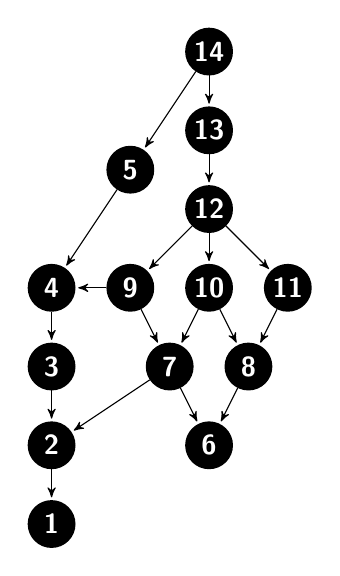
\begin{tikzpicture}[->,>=stealth',shorten >=1pt,auto,node distance=3cm,
  thick,main node/.style={circle,fill=blue!20,draw,font=\sffamily\Large\bfseries}]
  
  \foreach \place/\x in {{(0,0)/1}, {(0,1)/2},{(0,2)/3},{(0,3)/4}, {(1,4.5)/5}, {(2,1)/6}, {(1.5,2)/7},{(2.5,2)/8},{(1,3)/9},{(2,3)/10},{(3,3)/11},{(2,4)/12},{(2,5)/13},{(2,6)/14}}
  \node[arn_n] (a\x) at \place {\x};
%   Alice history
  \path[thin] (a14) edge (a5);
  \path[thin] (a5) edge (a4);
  \path[thin] (a4) edge (a3);
  \path[thin] (a3) edge (a2);
  \path[thin] (a2) edge (a1);
  \path[thin] (a9) edge (a4);
  \path[thin] (a7) edge (a2);
%   both history
  \path[thin] (a14) edge (a13);
  \path[thin] (a13) edge (a12);
  \path[thin] (a12) edge (a9);
  \path[thin] (a12) edge (a10);
  
  \path[thin] (a9) edge (a7);
  \path[thin] (a10) edge (a7);
%   Bob history
  \path[thin] (a12) edge (a11);
  \path[thin] (a11) edge (a8);
  \path[thin] (a10) edge (a8);
  \path[thin] (a7) edge (a6);
  \path[thin] (a8) edge (a6);
  \end{tikzpicture}
  }
  \caption{Main Graph} \label{fig:22a}
  \end{subfigure}%
 \begin{subfigure}[b]{0.3\textwidth}
  \centering
  \resizebox{0.9\textwidth}{!}{
  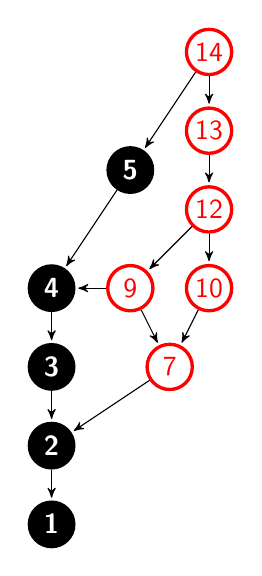
\begin{tikzpicture}[->,>=stealth',shorten >=1pt,auto,node distance=3cm,
  thick,main node/.style={circle,fill=blue!20,draw,font=\sffamily\Large\bfseries}]
  \foreach \place/\x in {{(0,0)/1}, {(0,1)/2}}
  \node[arn_n] (a\x) at \place {\x};
  
  
  \node[arn_n] (a5) at (1,4.5) {5};
  \node[arn_r] (a13) at (2,5) {13};
  \node[arn_r] (a14) at (2,6) {14};
  
  
  \node[arn_r] (a10) at (2,3) {10};
  \node[arn_r] (a7) at (1.5,2) {7};
  \node[arn_n] (a3) at (0,2) {3};
  
  \node[arn_r] (a9) at (1,3) {9};
  \node[arn_r] (a12) at (2,4) {12};
  \node[arn_n] (a4) at (0,3) {4};
  %   Alice history
  \path[thin] (a14) edge (a5);
  \path[thin] (a5) edge (a4);
  \path[thin] (a4) edge (a3);
  \path[thin] (a3) edge (a2);
  \path[thin] (a2) edge (a1);
  \path[thin] (a9) edge (a4);
  \path[thin] (a7) edge (a2);
%   both history
  \path[thin] (a14) edge (a13);
  \path[thin] (a13) edge (a12);
  \path[thin] (a12) edge (a9);
  \path[thin] (a12) edge (a10);
  
  \path[thin] (a9) edge (a7);
  \path[thin] (a10) edge (a7);
  \end{tikzpicture}
  }
  \caption{Alice's ancestors} \label{fig:22b}
\end{subfigure}
\begin{subfigure}[b]{0.3\textwidth}
\centering
  \resizebox{0.9\textwidth}{!}{
  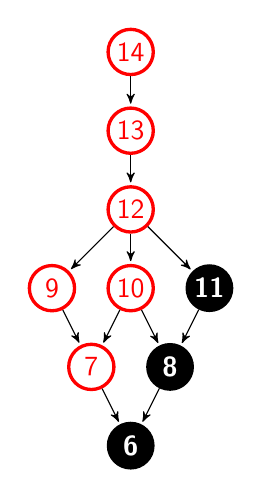
\begin{tikzpicture}[->,>=stealth',shorten >=1pt,auto,node distance=3cm,
  thick,main node/.style={circle,fill=blue!20,draw,font=\sffamily\Large\bfseries}]
%   
  \node[arn_n] (a6) at (2,1) {6};
  \node[arn_r] (a7) at (1.5,2) {7};
  \node[arn_n] (a8) at (2.5,2) {8};
  \node[arn_r] (a9) at (1,3) {9};
  \node[arn_r] (a10) at (2,3) {10};
  \node[arn_n] (a11) at (3,3) {11};
  \node[arn_r] (a12) at (2,4) {12};
  \node[arn_r] (a13) at (2,5) {13};
  \node[arn_r] (a14) at (2,6) {14};
  
%   both history
  \path[thin] (a14) edge (a13);
  \path[thin] (a13) edge (a12);
  \path[thin] (a12) edge (a9);
  \path[thin] (a12) edge (a10);
  
  \path[thin] (a9) edge (a7);
  \path[thin] (a10) edge (a7);
%   Bob history
  \path[thin] (a12) edge (a11);
  \path[thin] (a11) edge (a8);
  \path[thin] (a10) edge (a8);
  \path[thin] (a7) edge (a6);
  \path[thin] (a8) edge (a6);
  \end{tikzpicture}
  }
  \caption{Bob's ancestors} \label{fig:22c}
\end{subfigure}
\end{figure}
\end{frame}


\subsection{Hypothesis}
\begin{frame}

\begin{alertblock}{Hypothesis}
 \begin{itemize}
 \item \textbf{Each node has a unique hashable identifier}
 \item \textbf{At least one biggest common ancestor}
 \item \textbf{Any number of processes involved}
\end{itemize}
\end{alertblock}

\begin{exampleblock}{Objectives}
 \begin{itemize}
 \item Compute the difference between two Dags
  \item Optimized when the difference is small
  \item Minimise the complexity on both processes
  \item Minimise the quantity of information exchanged
 \end{itemize}
\end{exampleblock}
\end{frame}

\section{Results}

\subsection{Algorithm}
\begin{frame}
 \begin{block}{definition}
  \begin{itemize}
   \item Making a partition of a DAG into different \textbf{slices}.
   \item A slice $\mathcal S$ is paired with a \textbf{border} $\overline{ \mathcal S}$, such that $\forall x \in \mathcal S,\  \mathrm{pred}(x) \subset \mathcal S \cup \overline{\mathcal S}$
  \end{itemize}
   \end{block}
 \begin{figure}[H]
 
\centering
\resizebox{!}{5 cm}{
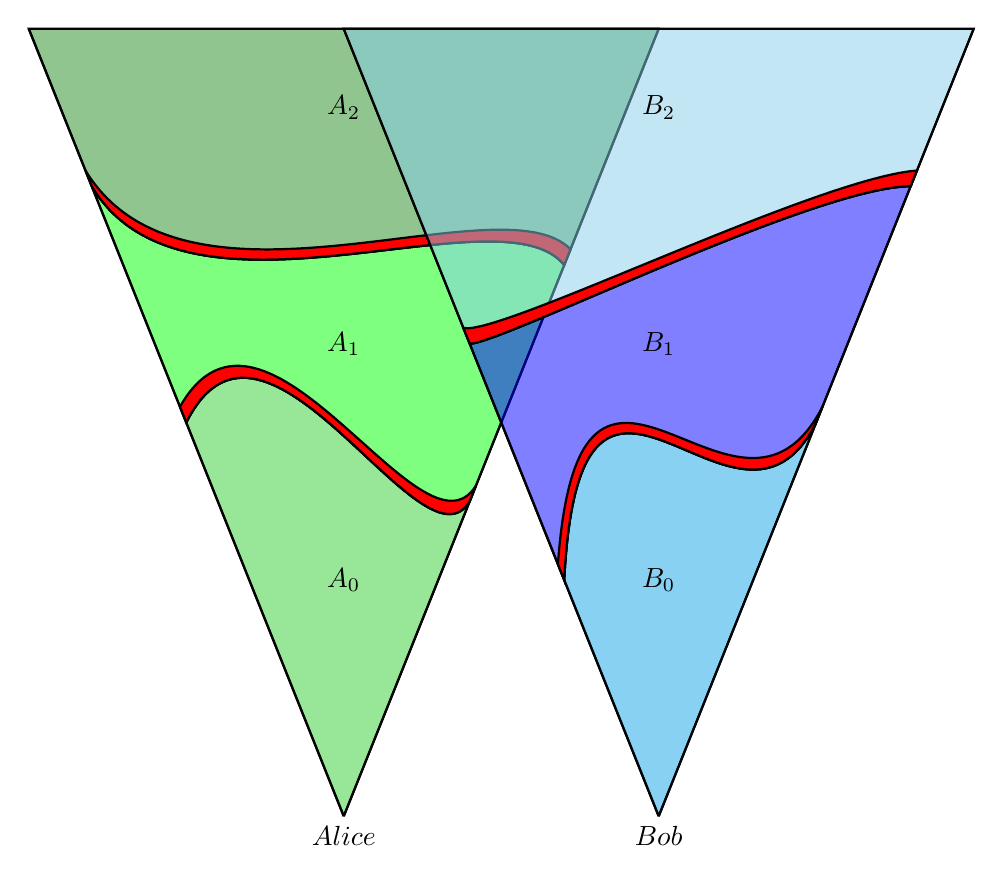
\begin{tikzpicture}
\begin{scope}
\coordinate[label=below:$Alice$] (A) at (0,0) ;
\coordinate (B) at (4,10);
\coordinate (C) at (-4,10);
\draw [thick] (A) -- (B) coordinate[pos = 0.4] (B1) {} coordinate [pos = 0.42] (B1b) {} coordinate[pos = 0.7] (B2) {} coordinate[pos = 0.72] (B2b) {};
\draw [thick] (B) -- (C) coordinate[pos = 0.5] (midBC) {};
\draw [thick] (A) -- (C) coordinate[pos = 0.5] (C1) {} coordinate [pos = 0.52] (C1b) {} coordinate[pos = 0.8] (C2) {} coordinate[pos = 0.82] (C2b) {};
\draw [thick, fill = LimeGreen,fill opacity = 0.5] (A) -- (B1) .. controls (1,3) and (-1,7) .. (C1) -- (A);
\draw [thick, fill = green,fill opacity = 0.5] (B1) .. controls (1,3) and (-1,7) .. (C1) -- (C2) .. controls (-2,6) and (2,8) .. (B2) -- (B1);
\draw [thick, fill = ForestGreen, fill opacity = 0.5] (C2) .. controls (-2,6) and (2,8) .. (B2) -- (B) -- (C) -- (C2);
\draw [thick, fill = red, fill opacity = 1] (B1b) .. controls (1,3.1) and (-1,7.1) .. (C1b) -- (C1) .. controls (-1,7) and (1,3) .. (B1) -- (B1b);
\draw [thick, fill = red, fill opacity = 1] (C2) .. controls (-2,6) and (2,8) .. (B2) -- (B2b) .. controls (2,8.1) and (-2,6.1) .. (C2b) -- (C2);
\draw [draw = none] (A) -- (midBC) node[pos = 0.3] {$A_0$} node[pos = 0.6] {$A_1$} node[pos = 0.9] {$A_2$};

\end{scope}
\begin{scope}[shift={(4cm,0cm)}]
\coordinate[label=below:$Bob$] (D) at (0,0);
\coordinate (E) at (4,10);
\coordinate (F) at (-4,10);
\draw [thick] (D) -- (E) coordinate[pos = 0.5] (E1) {} coordinate [pos = 0.52] (E1b) {} coordinate[pos = 0.8] (E2) {} coordinate[pos = 0.82] (E2b) {};
\draw [thick] (E) -- (F) coordinate[pos = 0.5] (midEF) {};
\draw [thick] (D) -- (F) coordinate[pos = 0.3] (F1) {} coordinate [pos = 0.32] (F1b) {} coordinate[pos = 0.6] (F2) {} coordinate[pos = 0.62] (F2b) {};
\draw [thick, fill = Cerulean,fill opacity = 0.5] (D) -- (E1) .. controls (1,3) and (-1,7) .. (F1) -- (D);
\draw [thick, fill = blue,fill opacity = 0.5] (E1) .. controls (1,3) and (-1,7) .. (F1) -- (F2) .. controls (-2,6) and (2,8) .. (E2) -- (E1);
\draw [thick, fill = SkyBlue, fill opacity = 0.5] (F2) .. controls (-2,6) and (2,8) .. (E2) -- (E) -- (F) -- (F2);
\draw [thick, fill = red, fill opacity = 1] (E1b) .. controls (1,3.1) and (-1,7.1) .. (F1b) -- (F1) .. controls (-1,7) and (1,3) .. (E1) -- (E1b);
\draw [thick, fill = red, fill opacity = 1] (F2) .. controls (-2,6) and (2,8) .. (E2) -- (E2b) .. controls (2,8.1) and (-2,6.1) .. (F2b) -- (F2);
\draw [draw = none] (D) -- (midEF) node[pos = 0.3] {$B_0$} node[pos = 0.6] {$B_1$} node[pos = 0.9] {$B_2$};
\end{scope}
\end{tikzpicture}
}
% \caption{Two processes sharing a part of their history and their decomposition in Slices and Borders} \label{fig:twoproc}
\end{figure}

\end{frame}

\begin{frame}[fragile]
 \frametitle{Exploration}
 \begin{exampleblock}{Signature}
 \begin{lstlisting}
  val explore : vertex list -> graph -> slice -> borders -> (graph * (vertex list))
 \end{lstlisting}
 \end{exampleblock}

 \begin{block}{Idea of the algorithm}
  \begin{enumerate}
\setbeamercovered{transparent}
\uncover<2-2>{\item Given a slice and borders the server explores its past and stop when it crosses a slice or a border}
\uncover<3-3>{\item The server computes the DAG $D$ of the successors of every nodes it found in slice.}
\uncover<4-4>{\item The server computes a list of "nodes of interest" from which it shall start again the exploration.}
\end{enumerate}
 \end{block}

%  val next_ring : vertex list -> graph list -> database -> database -> (graph * (vertex list))


\end{frame}

\begin{frame}
\begin{figure}[H]
\only<1>{
\begin{subfigure}[b]{0.5\textwidth}
\centering
  \resizebox{0.6\textwidth}{!}{
  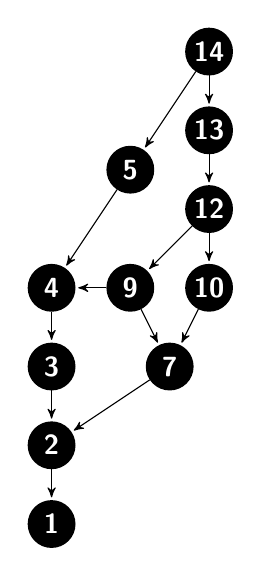
\begin{tikzpicture}[->,>=stealth',shorten >=1pt,auto,node distance=3cm,
  thick,main node/.style={circle,fill=blue!20,draw,font=\sffamily\Large\bfseries}]
  \foreach \place/\x in {{(0,0)/1}, {(0,1)/2}}
  \node[arn_n] (a\x) at \place {\x};
  
  
  \node[arn_n] (a5) at (1,4.5) {5};
  \node[arn_n] (a13) at (2,5) {13};
  \node[arn_n] (a14) at (2,6) {14};
  
  
  \node[arn_n] (a10) at (2,3) {10};
  \node[arn_n] (a7) at (1.5,2) {7};
  \node[arn_n] (a3) at (0,2) {3};
  
  \node[arn_n] (a9) at (1,3) {9};
  \node[arn_n] (a12) at (2,4) {12};
  \node[arn_n] (a4) at (0,3) {4};
  %   Alice history
  \path[thin] (a14) edge (a5);
  \path[thin] (a5) edge (a4);
  \path[thin] (a4) edge (a3);
  \path[thin] (a3) edge (a2);
  \path[thin] (a2) edge (a1);
  \path[thin] (a9) edge (a4);
  \path[thin] (a7) edge (a2);
%   both history
  \path[thin] (a14) edge (a13);
  \path[thin] (a13) edge (a12);
  \path[thin] (a12) edge (a9);
  \path[thin] (a12) edge (a10);
  
  \path[thin] (a9) edge (a7);
  \path[thin] (a10) edge (a7);
  \end{tikzpicture}
  }
  \caption*{Alice's ancestors}
\end{subfigure}%
}%
\only<2>{
\begin{subfigure}[b]{0.5\textwidth}
\centering
  \resizebox{0.6\textwidth}{!}{
 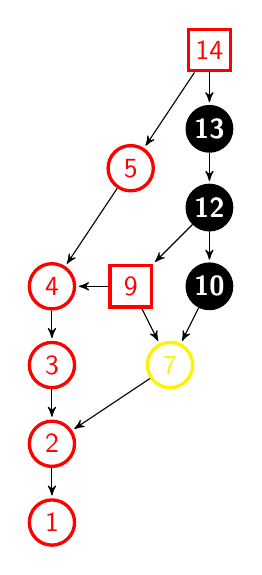
\begin{tikzpicture}[->,>=stealth',shorten >=1pt,auto,node distance=3cm,
  thick,main node/.style={circle,fill=blue!20,draw,font=\sffamily\Large\bfseries}]
  
  
  
  \node[arn_r] (a1) at (0,0) {1};
  \node[arn_r] (a2) at (0,1) {2};
  
  \node[arn_r] (a5) at (1,4.5) {5};
  \node[arn_n] (a13) at (2,5) {13};
  \node[arn_rs] (a14) at (2,6) {14};
  
  
  \node[arn_n] (a10) at (2,3) {10};
  \node[arn_y] (a7) at (1.5,2) {7};
  \node[arn_r] (a3) at (0,2) {3};
  
  \node[arn_rs] (a9) at (1,3) {9};
  \node[arn_n] (a12) at (2,4) {12};
  \node[arn_r] (a4) at (0,3) {4};
  
  %   Alice history
  \path[thin] (a14) edge (a5);
  \path[thin] (a5) edge (a4);
  \path[thin] (a4) edge (a3);
  \path[thin] (a3) edge (a2);
  \path[thin] (a2) edge (a1);
  \path[thin] (a9) edge (a4);
  \path[thin] (a7) edge (a2);
%   both history
  \path[thin] (a14) edge (a13);
  \path[thin] (a13) edge (a12);
  \path[thin] (a12) edge (a9);
  \path[thin] (a12) edge (a10);
  
  \path[thin] (a9) edge (a7);
  \path[thin] (a10) edge (a7);
  \end{tikzpicture}
  }
  \caption*{[1] Explore}
\end{subfigure}%
}%
\only<3>{
\begin{subfigure}[b]{0.5\textwidth}
\centering
  \resizebox{0.6\textwidth}{!}{
 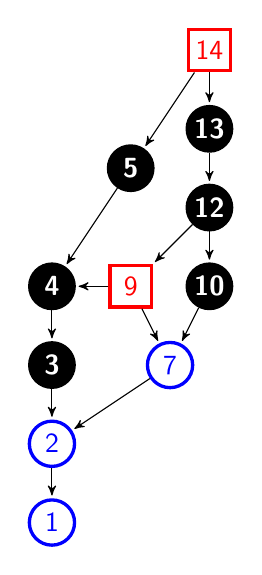
\begin{tikzpicture}[->,>=stealth',shorten >=1pt,auto,node distance=3cm,
  thick,main node/.style={circle,fill=blue!20,draw,font=\sffamily\Large\bfseries}]
  
  
  
  \node[arn_b] (a1) at (0,0) {1};
  \node[arn_b] (a2) at (0,1) {2};
  
  \node[arn_n] (a5) at (1,4.5) {5};
  \node[arn_n] (a13) at (2,5) {13};
  \node[arn_rs] (a14) at (2,6) {14};
  
  
  \node[arn_n] (a10) at (2,3) {10};
  \node[arn_b] (a7) at (1.5,2) {7};
  \node[arn_n] (a3) at (0,2) {3};
  
  \node[arn_rs] (a9) at (1,3) {9};
  \node[arn_n] (a12) at (2,4) {12};
  \node[arn_n] (a4) at (0,3) {4};
  
  %   Alice history
  \path[thin] (a14) edge (a5);
  \path[thin] (a5) edge (a4);
  \path[thin] (a4) edge (a3);
  \path[thin] (a3) edge (a2);
  \path[thin] (a2) edge (a1);
  \path[thin] (a9) edge (a4);
  \path[thin] (a7) edge (a2);
%   both history
  \path[thin] (a14) edge (a13);
  \path[thin] (a13) edge (a12);
  \path[thin] (a12) edge (a9);
  \path[thin] (a12) edge (a10);
  
  \path[thin] (a9) edge (a7);
  \path[thin] (a10) edge (a7);
  \end{tikzpicture}
  }
  \caption*{[2] Deal with nodes in Slice}
\end{subfigure}%
}%
\only<4>{
\begin{subfigure}[b]{0.5\textwidth}
\centering
  \resizebox{0.6\textwidth}{!}{
 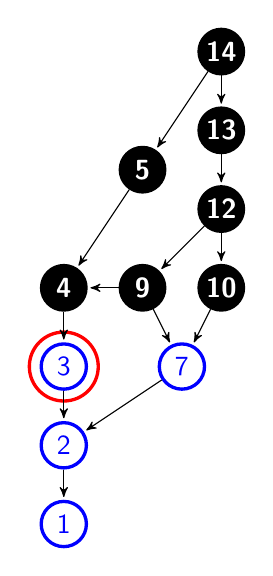
\begin{tikzpicture}[->,>=stealth',shorten >=1pt,auto,node distance=3cm,
  thick,main node/.style={circle,fill=blue!20,draw,font=\sffamily\Large\bfseries}]
  
  

  \node[arn_rb] (emph) at (0,2) {};
  \node[arn_b] (a1) at (0,0) {1};
  \node[arn_b] (a2) at (0,1) {2};
  
  \node[arn_n] (a5) at (1,4.5) {5};
  \node[arn_n] (a13) at (2,5) {13};
  \node[arn_n] (a14) at (2,6) {14};
  
  
  \node[arn_n] (a10) at (2,3) {10};
  \node[arn_b] (a7) at (1.5,2) {7};
  \node[arn_b] (a3) at (0,2) {3};
  
  \node[arn_n] (a9) at (1,3) {9};
  \node[arn_n] (a12) at (2,4) {12};
  \node[arn_n] (a4) at (0,3) {4};
%   \node[cloud, fill=gray!20, cloud puffs=16, cloud puff arc= 100,minimum width=2em, minimum height=2em, aspect=1] (cloud) at (5,2) {};

  %   Alice history
  \path[thin] (a14) edge (a5);
  \path[thin] (a5) edge (a4);
  \path[thin] (a4) edge (a3);
  \path[thin] (a3) edge (a2);
  \path[thin] (a2) edge (a1);
  \path[thin] (a9) edge (a4);
  \path[thin] (a7) edge (a2);
%   both history
  \path[thin] (a14) edge (a13);
  \path[thin] (a13) edge (a12);
  \path[thin] (a12) edge (a9);
  \path[thin] (a12) edge (a10);
  
  \path[thin] (a9) edge (a7);
  \path[thin] (a10) edge (a7);
  \end{tikzpicture}
  }
  \caption*{[3] Deal with nodes in Border}
\end{subfigure}%
}%
\only<5>{
\begin{subfigure}[b]{0.5\textwidth}
\centering
  \resizebox{0.6\textwidth}{!}{
 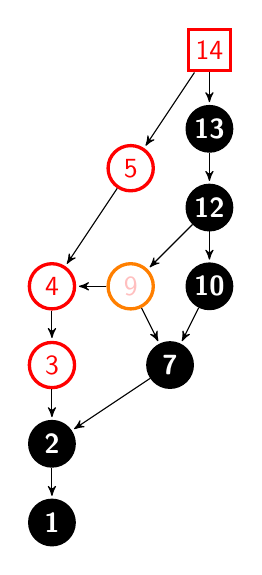
\begin{tikzpicture}[->,>=stealth',shorten >=1pt,auto,node distance=3cm,
  thick,main node/.style={circle,fill=blue!20,draw,font=\sffamily\Large\bfseries}]
  
  
  \node[arn_n] (a1) at (0,0) {1};
  \node[arn_n] (a2) at (0,1) {2};
  
  \node[arn_r] (a5) at (1,4.5) {5};
  \node[arn_n] (a13) at (2,5) {13};
  \node[arn_rs] (a14) at (2,6) {14};
  
  
  \node[arn_n] (a10) at (2,3) {10};
  \node[arn_n] (a7) at (1.5,2) {7};
  \node[arn_r] (a3) at (0,2) {3};
  
  \node[arn_t] (a9) at (1,3) {9};
  \node[arn_n] (a12) at (2,4) {12};
  \node[arn_r] (a4) at (0,3) {4};
%   \node[cloud, fill=gray!20, cloud puffs=16, cloud puff arc= 100,minimum width=2em, minimum height=2em, aspect=1] (cloud) at (5,2) {};

  %   Alice history
  \path[thin] (a14) edge (a5);
  \path[thin] (a5) edge (a4);
  \path[thin] (a4) edge (a3);
  \path[thin] (a3) edge (a2);
  \path[thin] (a2) edge (a1);
  \path[thin] (a9) edge (a4);
  \path[thin] (a7) edge (a2);
%   both history
  \path[thin] (a14) edge (a13);
  \path[thin] (a13) edge (a12);
  \path[thin] (a12) edge (a9);
  \path[thin] (a12) edge (a10);
  
  \path[thin] (a9) edge (a7);
  \path[thin] (a10) edge (a7);
  \end{tikzpicture}
  }
  \caption*{[1] Explore}
\end{subfigure}%
}%
\only<6>{
\begin{subfigure}[b]{0.5\textwidth}
\centering
  \resizebox{0.6\textwidth}{!}{
 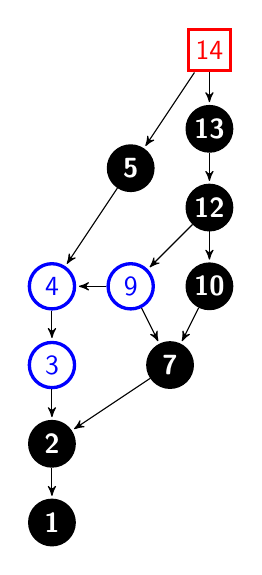
\begin{tikzpicture}[->,>=stealth',shorten >=1pt,auto,node distance=3cm,
  thick,main node/.style={circle,fill=blue!20,draw,font=\sffamily\Large\bfseries}]
  
  
  \node[arn_n] (a1) at (0,0) {1};
  \node[arn_n] (a2) at (0,1) {2};
  
  \node[arn_n] (a5) at (1,4.5) {5};
  \node[arn_n] (a13) at (2,5) {13};
  \node[arn_rs] (a14) at (2,6) {14};
  
  
  \node[arn_n] (a10) at (2,3) {10};
  \node[arn_n] (a7) at (1.5,2) {7};
  \node[arn_b] (a3) at (0,2) {3};
  
  \node[arn_b] (a9) at (1,3) {9};
  \node[arn_n] (a12) at (2,4) {12};
  \node[arn_b] (a4) at (0,3) {4};
%   \node[cloud, fill=gray!20, cloud puffs=16, cloud puff arc= 100,minimum width=2em, minimum height=2em, aspect=1] (cloud) at (5,2) {};

  %   Alice history
  \path[thin] (a14) edge (a5);
  \path[thin] (a5) edge (a4);
  \path[thin] (a4) edge (a3);
  \path[thin] (a3) edge (a2);
  \path[thin] (a2) edge (a1);
  \path[thin] (a9) edge (a4);
  \path[thin] (a7) edge (a2);
%   both history
  \path[thin] (a14) edge (a13);
  \path[thin] (a13) edge (a12);
  \path[thin] (a12) edge (a9);
  \path[thin] (a12) edge (a10);
  
  \path[thin] (a9) edge (a7);
  \path[thin] (a10) edge (a7);
  \end{tikzpicture}
  }
  \caption*{[2] Deal with nodes in Slice}
\end{subfigure}%
}%
\only<7>{
\begin{subfigure}[b]{0.5\textwidth}
\centering
  \resizebox{0.6\textwidth}{!}{
 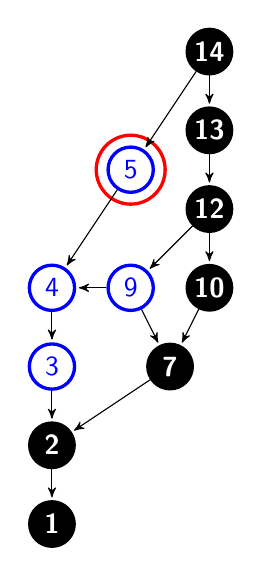
\begin{tikzpicture}[->,>=stealth',shorten >=1pt,auto,node distance=3cm,
  thick,main node/.style={circle,fill=blue!20,draw,font=\sffamily\Large\bfseries}]
  
  \node[arn_rb] (emph) at (1,4.5) {};
  \node[arn_n] (a1) at (0,0) {1};
  \node[arn_n] (a2) at (0,1) {2};
  
  \node[arn_b] (a5) at (1,4.5) {5};
  \node[arn_n] (a13) at (2,5) {13};
  \node[arn_n] (a14) at (2,6) {14};
  
  
  \node[arn_n] (a10) at (2,3) {10};
  \node[arn_n] (a7) at (1.5,2) {7};
  \node[arn_b] (a3) at (0,2) {3};
  
  \node[arn_b] (a9) at (1,3) {9};
  \node[arn_n] (a12) at (2,4) {12};
  \node[arn_b] (a4) at (0,3) {4};
%   \node[cloud, fill=gray!20, cloud puffs=16, cloud puff arc= 100,minimum width=2em, minimum height=2em, aspect=1] (cloud) at (5,2) {};

  %   Alice history
  \path[thin] (a14) edge (a5);
  \path[thin] (a5) edge (a4);
  \path[thin] (a4) edge (a3);
  \path[thin] (a3) edge (a2);
  \path[thin] (a2) edge (a1);
  \path[thin] (a9) edge (a4);
  \path[thin] (a7) edge (a2);
%   both history
  \path[thin] (a14) edge (a13);
  \path[thin] (a13) edge (a12);
  \path[thin] (a12) edge (a9);
  \path[thin] (a12) edge (a10);
  
  \path[thin] (a9) edge (a7);
  \path[thin] (a10) edge (a7);
  \end{tikzpicture}
  }
  \caption*{[3] Deal with nodes in Border}
\end{subfigure}%
}%
\only<8>{
\begin{subfigure}[b]{0.5\textwidth}
\centering
  \resizebox{0.6\textwidth}{!}{
 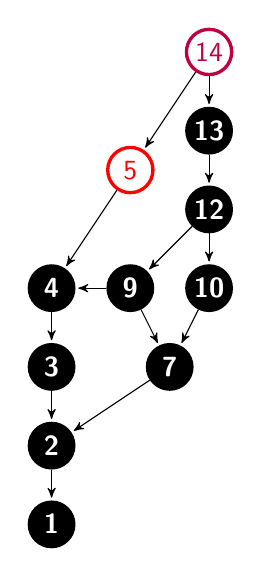
\begin{tikzpicture}[->,>=stealth',shorten >=1pt,auto,node distance=3cm,
  thick,main node/.style={circle,fill=blue!20,draw,font=\sffamily\Large\bfseries}]
  
  
  \node[arn_n] (a1) at (0,0) {1};
  \node[arn_n] (a2) at (0,1) {2};
  
  \node[arn_r] (a5) at (1,4.5) {5};
  \node[arn_n] (a13) at (2,5) {13};
  \node[arn_pu] (a14) at (2,6) {14};
  
  
  \node[arn_n] (a10) at (2,3) {10};
  \node[arn_n] (a7) at (1.5,2) {7};
  \node[arn_n] (a3) at (0,2) {3};
  
  \node[arn_n] (a9) at (1,3) {9};
  \node[arn_n] (a12) at (2,4) {12};
  \node[arn_n] (a4) at (0,3) {4};
%   \node[cloud, fill=gray!20, cloud puffs=16, cloud puff arc= 100,minimum width=2em, minimum height=2em, aspect=1] (cloud) at (5,2) {};

  %   Alice history
  \path[thin] (a14) edge (a5);
  \path[thin] (a5) edge (a4);
  \path[thin] (a4) edge (a3);
  \path[thin] (a3) edge (a2);
  \path[thin] (a2) edge (a1);
  \path[thin] (a9) edge (a4);
  \path[thin] (a7) edge (a2);
%   both history
  \path[thin] (a14) edge (a13);
  \path[thin] (a13) edge (a12);
  \path[thin] (a12) edge (a9);
  \path[thin] (a12) edge (a10);
  
  \path[thin] (a9) edge (a7);
  \path[thin] (a10) edge (a7);
  \end{tikzpicture}
  }
  \caption*{[1] Explore}
\end{subfigure}%
}%
\only<9>{
\begin{subfigure}[b]{0.5\textwidth}
\centering
  \resizebox{0.6\textwidth}{!}{
 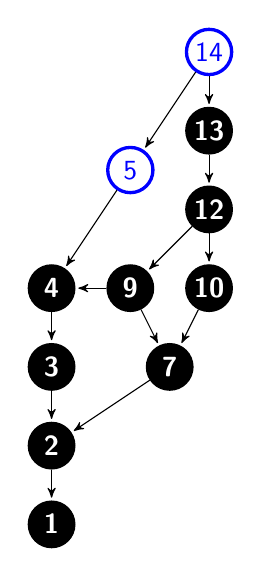
\begin{tikzpicture}[->,>=stealth',shorten >=1pt,auto,node distance=3cm,
  thick,main node/.style={circle,fill=blue!20,draw,font=\sffamily\Large\bfseries}]
  
  
  \node[arn_n] (a1) at (0,0) {1};
  \node[arn_n] (a2) at (0,1) {2};
  
  \node[arn_b] (a5) at (1,4.5) {5};
  \node[arn_n] (a13) at (2,5) {13};
  \node[arn_b] (a14) at (2,6) {14};
  
  
  \node[arn_n] (a10) at (2,3) {10};
  \node[arn_n] (a7) at (1.5,2) {7};
  \node[arn_n] (a3) at (0,2) {3};
  
  \node[arn_n] (a9) at (1,3) {9};
  \node[arn_n] (a12) at (2,4) {12};
  \node[arn_n] (a4) at (0,3) {4};
%   \node[cloud, fill=gray!20, cloud puffs=16, cloud puff arc= 100,minimum width=2em, minimum height=2em, aspect=1] (cloud) at (5,2) {};

  %   Alice history
  \path[thin] (a14) edge (a5);
  \path[thin] (a5) edge (a4);
  \path[thin] (a4) edge (a3);
  \path[thin] (a3) edge (a2);
  \path[thin] (a2) edge (a1);
  \path[thin] (a9) edge (a4);
  \path[thin] (a7) edge (a2);
%   both history
  \path[thin] (a14) edge (a13);
  \path[thin] (a13) edge (a12);
  \path[thin] (a12) edge (a9);
  \path[thin] (a12) edge (a10);
  
  \path[thin] (a9) edge (a7);
  \path[thin] (a10) edge (a7);
  \end{tikzpicture}
  }
  \caption*{[2] Deal with nodes in Slice}
\end{subfigure}%
}%
\only<10>{
\begin{subfigure}[b]{0.5\textwidth}
\centering
  \resizebox{0.6\textwidth}{!}{
 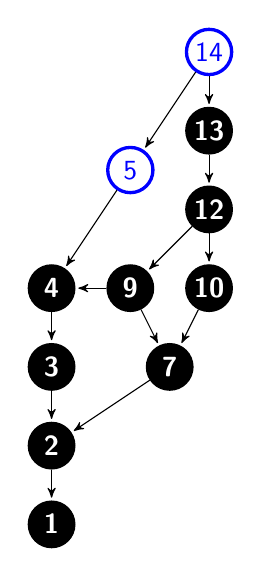
\begin{tikzpicture}[->,>=stealth',shorten >=1pt,auto,node distance=3cm,
  thick,main node/.style={circle,fill=blue!20,draw,font=\sffamily\Large\bfseries}]
  
  
  \node[arn_n] (a1) at (0,0) {1};
  \node[arn_n] (a2) at (0,1) {2};
  
  \node[arn_b] (a5) at (1,4.5) {5};
  \node[arn_n] (a13) at (2,5) {13};
  \node[arn_b] (a14) at (2,6) {14};
  
  
  \node[arn_n] (a10) at (2,3) {10};
  \node[arn_n] (a7) at (1.5,2) {7};
  \node[arn_n] (a3) at (0,2) {3};
  
  \node[arn_n] (a9) at (1,3) {9};
  \node[arn_n] (a12) at (2,4) {12};
  \node[arn_n] (a4) at (0,3) {4};
%   \node[cloud, fill=gray!20, cloud puffs=16, cloud puff arc= 100,minimum width=2em, minimum height=2em, aspect=1] (cloud) at (5,2) {};

  %   Alice history
  \path[thin] (a14) edge (a5);
  \path[thin] (a5) edge (a4);
  \path[thin] (a4) edge (a3);
  \path[thin] (a3) edge (a2);
  \path[thin] (a2) edge (a1);
  \path[thin] (a9) edge (a4);
  \path[thin] (a7) edge (a2);
%   both history
  \path[thin] (a14) edge (a13);
  \path[thin] (a13) edge (a12);
  \path[thin] (a12) edge (a9);
  \path[thin] (a12) edge (a10);
  
  \path[thin] (a9) edge (a7);
  \path[thin] (a10) edge (a7);
  \end{tikzpicture}
  }
  \caption*{[3] Deal with nodes in Border}
\end{subfigure}%
}%
\begin{subfigure}[b]{0.5\textwidth}
\centering
  \resizebox{0.6\textwidth}{!}{
  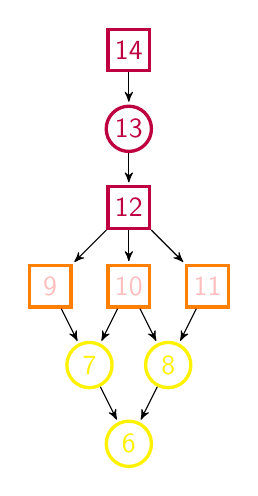
\begin{tikzpicture}[->,>=stealth',shorten >=1pt,auto,node distance=3cm,
  thick,main node/.style={circle,fill=blue!20,draw,font=\sffamily\Large\bfseries}]
%   
  \node[arn_y] (a6) at (2,1) {6};
  \node[arn_y] (a7) at (1.5,2) {7};
  \node[arn_y] (a8) at (2.5,2) {8};
  \node[arn_ts] (a9) at (1,3) {9};
  \node[arn_ts] (a10) at (2,3) {10};
  \node[arn_ts] (a11) at (3,3) {11};
  \node[arn_pus] (a12) at (2,4) {12};
  \node[arn_pu] (a13) at (2,5) {13};
  \node[arn_pus] (a14) at (2,6) {14};
  
%   both history
  \path[thin] (a14) edge (a13);
  \path[thin] (a13) edge (a12);
  \path[thin] (a12) edge (a9);
  \path[thin] (a12) edge (a10);
  
  \path[thin] (a9) edge (a7);
  \path[thin] (a10) edge (a7);
%   Bob history
  \path[thin] (a12) edge (a11);
  \path[thin] (a11) edge (a8);
  \path[thin] (a10) edge (a8);
  \path[thin] (a7) edge (a6);
  \path[thin] (a8) edge (a6);
  \end{tikzpicture}
  }
  \caption*{Bob's ancestors}

\end{subfigure}
\end{figure}
\end{frame}

\subsection{Bloom Filters}
\begin{frame}
 \frametitle{Bloom Filters}
 \begin{figure}[H]
 \resizebox{\linewidth}{!}{
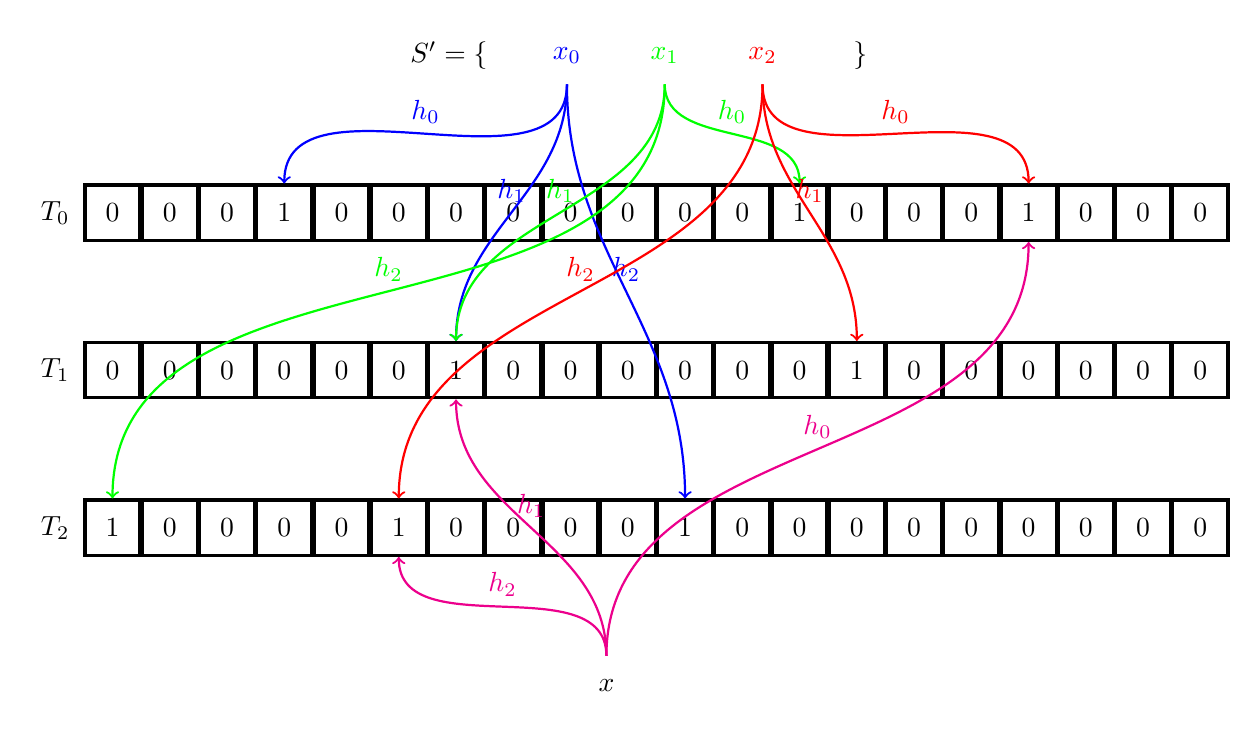
\begin{tikzpicture}
\tikzstyle{every path}=[very thick]

\edef\sizehash{0.7cm}
\tikzstyle{tmtape}=[draw,minimum size=\sizehash]

\begin{scope}[start chain=2 going right,node distance= 0.5cm]
    \node [on chain=2,tmtape,draw = none] {$S'=\{$};
    \node [on chain = 2,tmtape,draw = none] (x0) {\textcolor{blue}{$x_0$}};
    \node [on chain = 2,tmtape,draw = none] (x1) {\textcolor{green}{$x_1$}};
    \node [on chain = 2,tmtape,draw = none] (x2) {\textcolor{red}{$x_2$}};
    \node [on chain=2,tmtape,draw = none] {$\}$};
\end{scope}

\begin{scope}[shift={(-5cm,-2cm)},start chain=1 going right,node distance=-0.15mm]
    \node [on chain=1,tmtape,draw = none] {$T_0$};
    \node [on chain=1,tmtape] {$0$};
    \node [on chain=1,tmtape] {$0$};
    \node [on chain=1,tmtape] {$0$};
    \node [on chain=1,tmtape] (n0) {$1$};
    \node [on chain=1,tmtape] {$0$};
    \node [on chain=1,tmtape] {$0$};
    \node [on chain=1,tmtape] {$0$};
    \node [on chain=1,tmtape] {$0$};
    \node [on chain=1,tmtape] {$0$};
    \node [on chain=1,tmtape] {$0$};
    \node [on chain=1,tmtape] {$0$};
    \node [on chain=1,tmtape] {$0$};
    \node [on chain=1,tmtape] (n1) {$1$};
    \node [on chain=1,tmtape] {$0$};
    \node [on chain=1,tmtape] {$0$};
    \node [on chain=1,tmtape] {$0$};
    \node [on chain=1,tmtape] (n2) {$1$};
    \node [on chain=1,tmtape] {$0$};
    \node [on chain=1,tmtape] {$0$};
    \node [on chain=1,tmtape] {$0$};
\end{scope}

\begin{scope}[shift={(-5cm,-4cm)},start chain=1 going right,node distance=-0.15mm]
\node [on chain=1,tmtape,draw = none] {$T_1$};
    \node [on chain=1,tmtape] {$0$};
    \node [on chain=1,tmtape] {$0$};
    \node [on chain=1,tmtape] {$0$};
    \node [on chain=1,tmtape] {$0$};
    \node [on chain=1,tmtape] {$0$};
    \node [on chain=1,tmtape] {$0$};
    \node [on chain=1,tmtape] (n3) {$1$};
    \node [on chain=1,tmtape] {$0$};
    \node [on chain=1,tmtape] {$0$};
    \node [on chain=1,tmtape] {$0$};
    \node [on chain=1,tmtape] {$0$};
    \node [on chain=1,tmtape] {$0$};
    \node [on chain=1,tmtape] {$0$};
    \node [on chain=1,tmtape] (n4) {$1$};
    \node [on chain=1,tmtape] {$0$};
    \node [on chain=1,tmtape] {$0$};
    \node [on chain=1,tmtape] {$0$};
    \node [on chain=1,tmtape] {$0$};
    \node [on chain=1,tmtape] {$0$};
    \node [on chain=1,tmtape] {$0$};
\end{scope}
\begin{scope}[shift={(-5cm,-6cm)},start chain=1 going right,node distance=-0.15mm]
\node [on chain=1,tmtape,draw = none] {$T_2$};
    \node [on chain=1,tmtape] (n5) {$1$};
    \node [on chain=1,tmtape] {$0$};
    \node [on chain=1,tmtape] {$0$};
    \node [on chain=1,tmtape] {$0$};
    \node [on chain=1,tmtape] {$0$};
    \node [on chain=1,tmtape] (n6) {$1$};
    \node [on chain=1,tmtape] {$0$};
    \node [on chain=1,tmtape] {$0$};
    \node [on chain=1,tmtape] {$0$};
    \node [on chain=1,tmtape] {$0$};
    \node [on chain=1,tmtape] (n7) {$1$};
    \node [on chain=1,tmtape] {$0$};
    \node [on chain=1,tmtape] {$0$};
    \node [on chain=1,tmtape] {$0$};
    \node [on chain=1,tmtape] {$0$};
    \node [on chain=1,tmtape] {$0$};
    \node [on chain=1,tmtape] {$0$};
    \node [on chain=1,tmtape] {$0$};
    \node [on chain=1,tmtape] {$0$};
    \node [on chain=1,tmtape] {$0$};
\end{scope}
\begin{scope}[shift={(2cm,-8cm)},start chain=1 going right,node distance=-0.15mm]
\node [on chain=1,tmtape,draw = none] (x) {$x$};
\end{scope}

\draw[->,blue,thick] (x0.south) to[out=270,in=90] node[midway,above] {$h_0$} (n0.north);
\draw[->,blue,thick] (x0.south) to[out=270,in=90] node[midway,above] {$h_1$} (n3.north);
\draw[->,blue,thick] (x0.south) to[out=270,in=90] node[midway,above] {$h_2$} (n7.north);
\draw[->,green,thick] (x1.south) to[out=270,in=90] node[midway,above] {$h_0$} (n1.north);
\draw[->,green,thick] (x1.south) to[out=270,in=90] node[midway,above] {$h_1$} (n3.north);
\draw[->,green,thick] (x1.south) to[out=270,in=90] node[midway,above] {$h_2$} (n5.north);
\draw[->,red,thick] (x2.south) to[out=270,in=90] node[midway,above] {$h_0$} (n2.north);
\draw[->,red,thick] (x2.south) to[out=270,in=90] node[midway,above] {$h_1$} (n4.north);
\draw[->,red,thick] (x2.south) to[out=270,in=90] node[midway,above] {$h_2$} (n6.north);


\draw[->,magenta,thick] (x.north) to[out=90,in=270] node[midway,above] {$h_0$} (n2.south);
\draw[->,magenta,thick] (x.north) to[out=90,in=270] node[midway,above] {$h_1$} (n3.south);
\draw[->,magenta,thick] (x.north) to[out=90,in=270] node[midway,above] {$h_2$} (n6.south);
\end{tikzpicture}
}
\caption{Inserting and testing the membership in a Bloom Filter, $x$ is a false positive} \label{fig:fp}
\end{figure}
\end{frame}

\subsection{Asymptotic Behavior and False Positive}
\frametitle{Asymptotic Behavior and False Positive}
\begin{frame}
 \begin{alertblock}{Size Grow indefinitely}
  We drop $\frac{1}{4}$ of the Slices and Borders when too big (Half of last half). 
  \begin{itemize}
   \item Bounded Memory
   \item Still efficient for small difference
   \item Loss of efficient for big difference
  \end{itemize}
 \end{alertblock}
 \begin{alertblock}{False Positive}
 \begin{itemize}
  \item In Slice : Client realizes directly and ask the server again
  \item In Borders : Client can not realize and send all slices until it realizes
 \end{itemize}

\end{alertblock}
\end{frame}

\subsection{Evaluation}
\begin{frame}
\frametitle{Evaluation}
 \begin{figure}[H]
  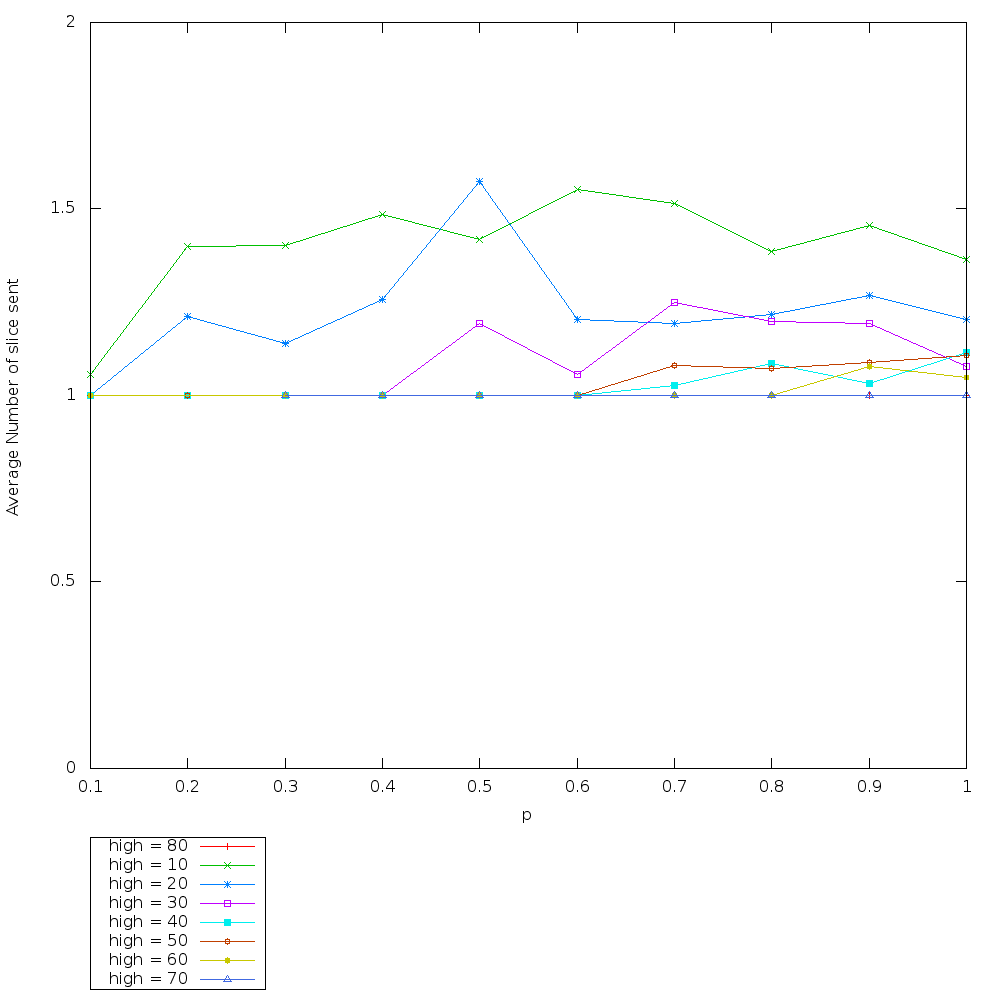
\includegraphics[height=7cm]{./image/slicesent/Nb_sent_slice.png}
 \end{figure}
\end{frame}

\section{Conclusion}
\begin{frame}
 \begin{exampleblock}{Conclusion}
  \begin{itemize}
   \item Very few false positive
   \item A small amount of information exchanged (an average of $20\times 320 \times 1.3$ bits in our example)
   \item A fast and incremental method on the client side, a linear (in the size of the difference) complexity on the server side.
   \item The server is memory free regarding a particular client.
  \end{itemize}
  \end{exampleblock}

\end{frame}


\end{document}
